\documentclass[10pt, twocolumn]{article}

%设置页边距
\usepackage{geometry}
\geometry{left=2.5cm,right=2.5cm,top=2.5cm,bottom=2.5cm}

%地址链接支持
\usepackage{hyperref}

%页眉页脚
\usepackage{fancyhdr}
\pagestyle{fancy}
\lhead{隔空画字}
\rhead{实验报告}

%设置字体
\usepackage[no-math]{fontspec}
\usepackage{xunicode}
\usepackage{xltxtra}
\usepackage{amsmath,amssymb, esint}
\usepackage[indentfirst=false,slantfont,boldfont]{xeCJK}
\setCJKmainfont[ItalicFont={Xingkai SC Light}, BoldFont={Songti SC Bold}]{Songti SC Light}
\setCJKsansfont{Lantinghei SC Demibold}
\setCJKmonofont{Songti SC Regular}

%设置换行缩进
\usepackage{indentfirst}

%行距
\linespread{1.2}

\usepackage{multirow}

\usepackage{xcolor}
\usepackage{caption}
\usepackage{float}
\usepackage{cite}

\begin{document}

\title{\textsf{隔空画字交互方式实验报告}}

\author{
徐炜杰\thanks{\href{mailto:xuweijie1995@sina.com}{xuweijie1995@sina.com}}\quad
韩旭\thanks{\href{mailto:thu.hanxu13@gmail.com}{thu.hanxu13@gmail.com}}
}


\date{2016年1月}
\renewcommand{\contentsname}{\textbf{目录}}
\renewcommand{\figurename}{\textbf{图}}
\renewcommand{\tablename}{\textbf{表}}

\twocolumn[
  \begin{@twocolumnfalse}
	\maketitle
  \end{@twocolumnfalse}
]


\section{简介}

在与传统的设备进行人机交互的过程中,在文本内容的输入方面,采取的方案通常有如下几种:通过键盘输入字符以构成文本的输入,对于中文之类的非字母语言则辅助以输入法进行交互;通过手写板或者触屏的方式直接将文字内容写在设备上,辅助以识别算法进行交互。事实上,这两种方式发展到如今已经十分成熟、可靠且高效了,尤其是在移动设备端上,对这两种方式的依赖程度更高。输入法的智能技术与模糊输入技术以及手写识别算法精度与速度的提升也使得这两者的交互过程更为舒畅。

同样传统的文本交互方式也具有一些不足。从键盘方面来讲,熟练掌握手机键盘输入的使用者,在文本内容的交互输入上是十分高效的,但前提是要十分熟悉输入法的规则以及键盘的具体结构,对于中文的输入来说,高效的输入更大程度上是依赖对输入法的熟悉程度来说的。但不是所有人都对输入法有充足的了解或者对键盘本身有足够的熟悉,而对于中年以及中年以上的人群,通常是无法操作键盘使用输入法进行文本交互的,而且很难有拼音输入的概念,部分方言地区拼音输入法会出现无法映射的问题,学习成本相对较高。

触屏的手写方式是对上述键盘问题的一种交互补偿,手写本身与键盘相比在速度和准确度上都不占有优势,其本身最有意义的一点在于学习成本极低,而且对于很多设备,受限于尺寸或者本身就无法很好的支持键盘,触屏将输入与输出交互融为一体更加的适应场景。而我们的设想就是更进一步,脱离实体的手写板或者触摸屏来进行手写输入,使得输入环境得到更大程度上的自由化,比较典型的就是本文讨论的隔空画字来进行输入,这就是我们的设计交互的基本概念和方式。 


\section{任务分析}

	脱离物理硬件设备来进行悬空手写,与传统的手写方式比较而言,优势在于简化输入设备,交互的活动范围更大,存在的基本问题也与此相关,在于缺乏有效的反馈激励,长时间且需要精度的书写模式是不适用这样的模式的,所以我们提出的设备环境与使用方式定位为小范围内容输入,支持手写设备以及键盘输入的可能性比较低的情况下,例如与电气设备进行交互。

	实现这样一个交互系统,总体上而言,需要完成三项核心任务。第二项是如何进行有效的手势数据收集以及处理,并将这些离散的数据整合成之后需要的特征集合。第二项任务是如何在有限的时间内,将任务一整合之后的特征集合识别成其对应的字符。第三项任务是如何有效的将任务二识别出来的结果反馈给系统的前台以及交互的用户,并且在整体系统运行期间实时反馈给用户当前的手写情况。

	\subsection{数据收集}

	对用户的手写过程进行收集要有效的解决两个问题,第一个是如何将输入的字符区分开来。传统的基于触碰设备的手写输入方式就有这样一个问题,不是所有的字符都是可以一笔画解决的,一个字符可能需要间断的几笔来刻画,因而区分两个字符之间的笔画间隔以及一个字符内连续的几个笔画的间隔是一个棘手的问题。传统的解决方案是通过间隔时间来解决的,通过设置一个时间间隔阈值来区分一个字符是否已经输入完毕了。这个问题对于脱离触摸板的隔空手写而言更为复杂,触摸板只需要记录触压的记录就可以得到书写轨迹的每一个笔画,但在真实空间里手指的轨迹必然是连续的,笔画本身的间断就很难区分,字符之间的间隔就更为复杂了。我们的解决方案是用手势来进行区分,每次向下微微拍动示意输入开始,结束的时候再向下微微拍动示意输入结束。这样的输入方式,相比于时间阈值而言更加快速和准确,也比较适应隔空输入无法区分笔画间断的特性。

	\begin{figure}[htb]
	\centering
	\begin{minipage}[t]{0.8\linewidth}
	\centering
	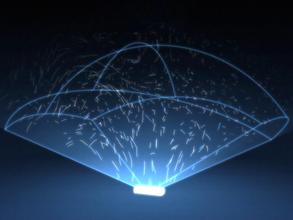
\includegraphics[height=4cm]{leapmotion.jpg}
	\caption{Leap Motion}
	\label{fig: sample_cnn}
	\end{minipage}
	\end{figure}

	对于手势的位置抓取以及手势的判断,我们采用了Leap Motion来解决需求。Leap Motion是面向PC以及Mac的体感控制器制造公司Leap于2013年2月27日发布的体感控制器,其基本功能在于可以追踪全部的10只手指的轨迹,精度可以达到1/100毫米。可以在其控制的一英尺宽的立方体中进行操作,且监控动作的空间视场宽幅达到了150度,如图1。通过每秒200帧的速度追踪操作者的手部移动,并可以在屏幕上与每次移动进行同步。	

	第二个问题是如何将三维的轨迹投影到二维。因为投影的面可以很多,但只有将所有的三维坐标投影到最接近书写状态的平面才是最容易进行识别的,因为在投影的过程中书写的轨迹或多或少会发生形变。由于三点确定一个平面,如果在不计时间成本的情况下,我们可以枚举任意的三个节点,构成一个平面,然后通过计算其余所有节点到这个平面的距离之和能衡量这个平面的质量。很明显,距离和最小的平面是最适宜用来映射并进一步去识别的选择。但事实上,这样的算法效率低下,具有时间上的致命局限。我们随机取出一部分节点进行采样,从其中选取一个局部最优的平面来进行识别,虽然仍然存在问题但是很好的做好了时间与效果的平衡。

	\subsection{数据识别}

	对于如何将输入的灰度图识别为对应的符号,我们采用了一种稳定且有效的算法。我们采用公开的手写识别数据集作为训练数据,通过卷积神经网络(CNN)来构建一个手写符号的分类器。在数据集的选择上,我们采用了MNIST手写识别数据集,这是一个应用比较广泛且质量比较可靠的数据集,比较好地符合了我们的实际需求。对于卷积神经网络的实现,我们采用了开源深度学习框架theano来构建我们需要的网络,theano与numpy的结合较为紧密,能够进行极具效率的训练和测试。具体关于MNIST与theano的说明可以详见附录链接。


	\begin{figure}[htb]
	\centering
	\begin{minipage}[t]{1\linewidth}
	\centering
	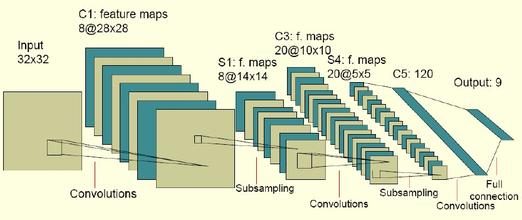
\includegraphics[width=8cm]{cnn1.jpg}
	\caption{cnn结构}
	\label{fig: sample_cnn}
	\end{minipage}
	\end{figure}

	卷积神经网络的基本框架分为卷积层,亚采样层,全连接层(如图2所示)。卷积层将输入的灰度图看作一个输入向量,采用一个滑动窗口不断滑动取样提取特征,特征的表现形式为局部灰度图的向量,然后通过矩阵进行一次线性变换,从而得到一个新的特征向量。由于卷积层每次采样都会得到一个特征向量,亚采样层会对这些卷积层得到的特征向量进行压缩,具体的操作就是选取每个维度上最大值或者最小值作为代表,并通过tanh或者sigmod函数进行归一化,输出的结果就变为尺寸稍小的一张灰度图。全连接层是在最后套接一个softmax,使得网络的输出向量能够得到输入向量对应每种分类情况的具体能量函数,从而确定输入的分类。

	\begin{figure}[htb]
	\centering
	\begin{minipage}[t]{1\linewidth}
	\centering
	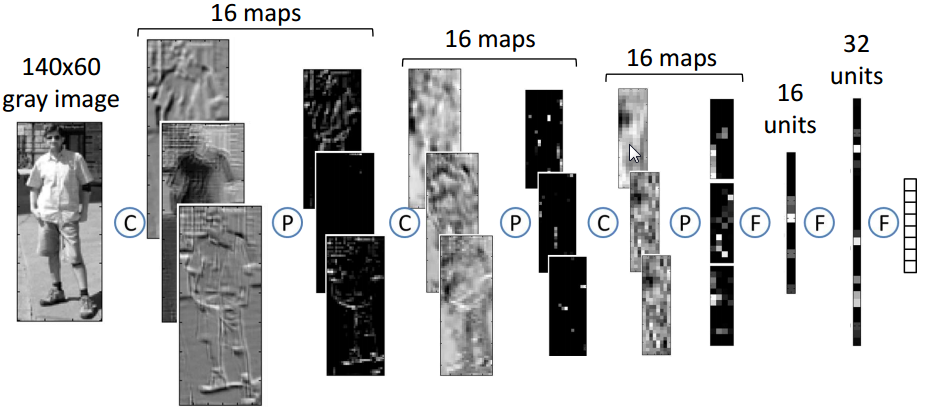
\includegraphics[width=8cm]{cnn2.png}
	\caption{cnn案例}
	\label{fig: sample_cnn}
	\end{minipage}
	\end{figure}

	图3就是一个典型的卷积神经网络对图片的特征压缩过程,只是最后没有全连接层进行分类算法。

	\subsection{数据反馈}

	如何将输入结果以及输入过程中的情况反馈给前台,我们的设计思路是采用两块屏幕区域来解决。两块反馈区域分别设计为交互反射区和结果投射区。交互反射区的作用是实时的将输入压缩成二维平面并在该区域上反馈出来,用以指导用户更加精确的进行手写输入。结果投射区就是将以往识别的结果投射到前台上。相比前两个任务,这个任务在实现上并没有过多的技术细节,但是其对整体交互感的影响是十分重大的。反馈区的情况可以参照图4

	\begin{figure}[htb]
	\centering
	\begin{minipage}[t]{1\linewidth}
	\centering
	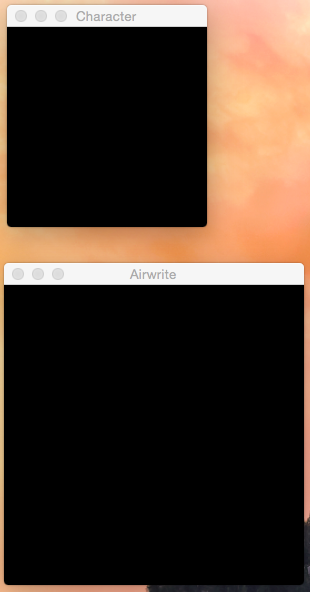
\includegraphics[width=4cm]{a}
	\caption{反射区域}
	\label{fig: sample_cnn}
	\end{minipage}
	\end{figure}


\section{框架描述}
	我们的实验过程中,通过使用Leap Motion来扑捉手势的坐标及状态,从而能够与后台的设备建立起简易的交互,并根据交互给予用户适当的反馈。我们的实现框架一共有三层。第一层为输入层,主要用来接收Leap Motion的数据输入。由于Leap Motion的采集的输入数据是一个三维坐标系的节点集合,而书写是建立在二维平面上的,所以需要算法进行映射压缩。第二层就是执行这些功能的映射层,用以将节点的踪迹映射压缩到一个二维平面上去。第三层为识别层,用以将第二层的输入平面识别为对应得字符,并从后台对前端进行反馈。

\begin{figure}[htb]
\centering
\begin{minipage}[t]{1\linewidth}
\centering
\includegraphics[height=8cm]{structure.png}
\caption{总体框架}
\label{fig: sample_cnn}
\end{minipage}
\end{figure}



\begin{figure}[htb]
\centering
\begin{minipage}[t]{1\linewidth}
\centering
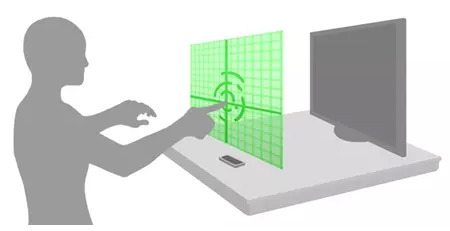
\includegraphics[width=8cm]{input.jpg}
\caption{输入层}
\label{fig: sample_cnn}
\end{minipage}
\end{figure}



\begin{figure}[htb]
\centering
\begin{minipage}[t]{1\linewidth}
\centering
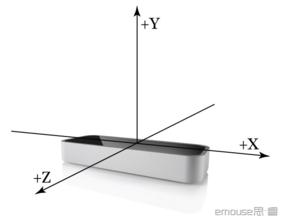
\includegraphics[width=8cm, height = 6cm]{map.jpg}
\caption{映射层}
\label{fig: sample_cnn}
\end{minipage}
\end{figure}

	识别层以映射层输出的$28 \times 28$的灰度点阵作为交互系统第三识别层的输入,其中采用了卷积神经网络算法来进行操作。对于卷积神经网络的参数,Convolution层我们选择了相对传统的$3 \times 3$的采样窗口。


\begin{figure}[htb]
\centering
\begin{minipage}[t]{1\linewidth}
\centering
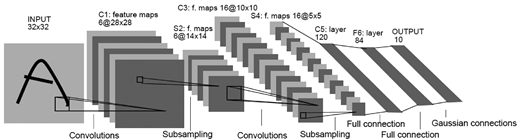
\includegraphics[width=8cm]{cnn.png}
\caption{识别层}
\label{fig: sample_cnn}
\end{minipage}
\end{figure}



\section{实验方法}
	
	围绕我们设计的交互目的,我们将整体任务划分为三个子任务,并分别进行实验:对输入时间的衡量,识别准确率的衡量,设备给出反馈时间的衡量。
	
	\subsection{参与者情况}
	
	\subsection{实验环境}

	\subsection{实验任务}
	
	针对实验中我们提出的三个子任务,我们设立了对应的三个实验分别进行测试。
	实验一是针对输入时间的衡量,我们要求实验参与者连续手写数字0到9,然后用完成任务所花费的时间进行度量,对于输入过程中的输入差错我们也将其也计入测量时间内。实验一同时也进行反馈效率的测试,对于每个测试参与者,我们要求其在有交互反射区的情况下进行有反馈输入试验,也要求其在没有交互反射区的情况下进行无反馈输入试验,以此来对比反馈机制对隔空手写输入的影响。
	
	试验二是针对识别准确率的衡量,我们针对系统能够进行识别的字符类型,数字0到9,小写字母a到z,大写字母A到Z分别进行了准确率测试。测试集一部分来源于公开的手写测试数据集,另一部分由测试参与者手写生成。对于识别率,我们以hit 1 与 hit 4 来衡量。hit 1 的意义是测试正确结果落在最优的分类结果上的比例,hit 4 的意义是测试正确结果落在前四优的分类结果中的比例。
	
	实验三是针对反应时间的衡量。该实验主要测试从输入完成到输入结果被反馈出来的时间,并收集用户对反馈时间的主观评估,用以探究反应时间对隔空手写输入这种交互方式的交互影响。

	\subsection{实验过程及方法}

	实验一,我们要求测试者使用我们搭建的交互设备隔空手写输入数字0到9。实验一共进行两轮,第一轮0到9输入,第二轮9到0输入。每轮输入分两次进行。第一轮的第一次是在关闭交互反射区的情况下进行输入,第二次是在打开交互反射区的情况下进行输入。第二轮则先在有交互反射区的情况下进行输入,再在没交互反射区的情况下进行输入。我们用两轮的平均用时来作为实验结果,并计算出输入每个字符的平均用时。关于两轮输入之间的时间间隔,我们设置了5分钟的休息时间,而每轮中的两次输入则是连续进行的,这样主要用来避免第一轮的熟练度会对第二轮实验造成干扰。


	实验二,我们在收集完测试集合之后直接使用卷积神经网络训练出来的模型进行测试。测试过程为针对每个数字和字母分别进行分类识别,从而算出所有符号的识别准确率。关于识别的准确率,我们采用 hit 1 与 hit 4 两套识别机制来进行识别,同时涵盖了精确性以及有效覆盖性的度量。这块内容与交互主体没有直接相关,为脱离测试者额外完成的实验,所以没有具体关于实验者的实验设置。

	实验三,我们在交互系统中加入了后台计时,用以度量每次从输入完成到输出反馈的时间间隔,我们用累计符号的输入总间隔时间求平均来衡量反应时间。另外在实验完成时我们收集用户对反应时间的主观反馈,用以与反应时间进行对照,以便从中发现问题。这块不会涉及到用户直接交互的问题,在实验一完成的过程中,该项实验同时完成实验数据的收集,所以没有具体关于实验者的实验设置。


\section{实验结果}

\section{结果讨论}
从实验的结果来看,预先设想的交互方式在平台上得到了一定的呈现与验证,脱离硬件进行文本输入的方式在可行度得到了证实,预先设想的效果也得到了有效的实现。同样,通过交互方式的实现以及对应的实验,我们也发现了影响隔空手写交互的一些具体因素。

隔空手写的一些特性:

第一,输入方式更为自由。相比传统的基于触碰硬件的手写输入交互方式,我们前文提到对手写设备产生的限制进行突破在我们的实验中得到了很好的体现。我们在实际操作中虽然需要将三维的输入数据压缩成二维的输入特征进行识别,但三维空间本身相比于二维空间,其自由度要大的多,虽然没有突破识别上对维度的限制,但却提升了交互的自由度。所以,虽然我们受限于Leap Motion设备本身的精度以及设计问题,但就实现效果来看,隔空的手写输入在操作范围和输入方式上都有了很大的提升。无论是水平面,竖直面还是各种空间中的复杂平面,输入的内容都能够被很好的检测与识别,并且从实验三来看,识别的准确率还是相对较高的。因而,该种交互的有效性在此有了一些体现。

第二,交互设备本身的构建更为自由。对于传统基于触控硬件的手写输入交互,设备本身需要有一定的面积以支持触控设备的安置。在我们的实现中,我们只使用了设备Leap Motion进行输入的采集,其余所涉及到的只有后台的计算资源。这样的简单设备配置就可以满足很大程度上的输入交互了,所以脱离触碰设备进行隔空的手写输入对硬件设备的简化也是十分有效的。对于一些有外观形状以及大小尺寸限制的设备,无需冗杂设备的隔空手写是一种十分有效的交互机制,能使得这些设备的交互得到极大丰富。

对于影响交互感的因素,大体有两点:

第一,该交互方式需要良好的反馈机制。正如我们预先设想到所存在的反馈机制问题,在隔空手写识别实验中得到了体现。从反馈机制拓展出去看,用笔书写、基于传统硬件设备的手写输入和我们提出的脱离硬件隔空进行手写输入,交互过程中的反馈是逐级下降的,即操作导致的疲劳度会逐级增加,这会影响交互的效率。而根据我们对实验者疲劳度的收集情况来看,实验情况与推测状况是一致的。根据这点,我们在实验一中进一步采用了无反馈机制以及有反馈机制分别进行实验并进行时间以及正确率的对比。可以发现,在加入反馈机制之后,正确率以及交互的速度都有了显著的提高。

第二,脱离硬件进行手写输入,影响交互舒适度的很大一个因素在于处理输入过程中发生的差错。在实验二中,我们可以发现,在有出错情况下,平均的输入时间被大比例的拉长,这种情况也是极其容易理解的。对于键盘输入,一但输入出现了差错,退格键就可以消除差错,再输入进同样内容也很简单。对于基于触屏硬件的手写输入,退格这样的功能往往也是脱离手写本身的。而在我们提出的交互机制中,对差错的处理是相对复杂的,这意味着在输入突然遭受错误中断时,交互的流畅度会受到不小的影响。因而,对交互异常的处理机制也是影响该种交互方式的重要因素,需要提出相应的解决方案。


\section{附录}



\end{document}





